% Compile:
%   pdflatex report.tex
% or:
%   latexmk -pdf report.tex
%
% Notes:
% - This PDF includes plots rendered with pgfplots (no external images required).
% - For interactive plots + one-click PNG/SVG exports, open `plots/report_graphs.html`.

\documentclass[11pt]{article}

\usepackage[margin=1in]{geometry}
\usepackage{microtype}
\usepackage{amsmath}
\usepackage{booktabs}
\usepackage{graphicx}
\usepackage{siunitx}
\usepackage{enumitem}
\usepackage{xcolor}
\usepackage{hyperref}
\usepackage{pgfplots}
\usepackage{subcaption}

\pgfplotsset{compat=1.18}
\sisetup{detect-weight=true, detect-family=true}
\hypersetup{
  colorlinks=true,
  linkcolor=blue!60!black,
  urlcolor=blue!60!black,
  citecolor=blue!60!black
}

% -----------------------------
% Key numbers (auto-copied from results_all.csv / REPORT.md as of 2026-03-11)
% -----------------------------
\newcommand{\NTotal}{597{,}928}
\newcommand{\NTrain}{418{,}549}
\newcommand{\NVal}{89{,}689}
\newcommand{\NTest}{89{,}690}

% Robustness: eval_suite (full features)
\newcommand{\AnnRandRmseMean}{0.1420}
\newcommand{\AnnRandRmseStd}{0.0036}
\newcommand{\AnnRandAccMean}{92.64}
\newcommand{\AnnRandAccStd}{0.31}

\newcommand{\HedRandRmseMean}{0.2446}
\newcommand{\HedRandRmseStd}{0.0030}
\newcommand{\HedRandAccMean}{87.76}
\newcommand{\HedRandAccStd}{0.10}

\newcommand{\AnnTimeRmseMean}{0.3146}
\newcommand{\AnnTimeRmseStd}{0.0365}
\newcommand{\AnnTimeAccMean}{82.78}
\newcommand{\AnnTimeAccStd}{2.35}

\newcommand{\HedTimeRmseMean}{0.5947}
\newcommand{\HedTimeRmseStd}{0.0162}
\newcommand{\HedTimeAccMean}{69.35}
\newcommand{\HedTimeAccStd}{1.09}

% DeepFM full-train (3 seeds: 0/1/42)
\newcommand{\DeepRandRmseMean}{0.1708}
\newcommand{\DeepRandRmseStd}{0.0085}
\newcommand{\DeepRandAccMean}{91.22}
\newcommand{\DeepRandAccStd}{0.51}

\newcommand{\DeepTimeRmseMean}{0.3533}
\newcommand{\DeepTimeRmseStd}{0.0107}
\newcommand{\DeepTimeAccMean}{75.74}
\newcommand{\DeepTimeAccStd}{1.51}

% Best single runs (full train, full features)
\newcommand{\BestAnnRunName}{\texttt{full\_deep4\_bs512\_lr4e-3\_do0.1\_wd1e-3}}
\newcommand{\BestAnnTestRmse}{0.1433}
\newcommand{\BestAnnTestAcc}{92.62}

\newcommand{\BestDeepfmRunName}{\texttt{deepfm\_best\_fulltrain\_seed1}}
\newcommand{\BestDeepfmTestRmse}{0.1621}
\newcommand{\BestDeepfmTestAcc}{91.80}

\newcommand{\BestHedTestRmse}{0.2428}
\newcommand{\BestHedTestAcc}{87.74}

\title{House Price Modeling (Hedonic vs Neural Tabular Models)\\
\large Experimental Evaluation, Robustness, and Feature Insights}
\author{RPSAps360 Project}
\date{March 11, 2026}

\begin{document}
\maketitle

\begin{abstract}
This report summarizes an end-to-end pipeline for predicting \texttt{TransactionPrice} from housing transaction data, compares a classic hedonic regression baseline to multiple neural tabular models (ANN, FM, DeepFM, TabNet), and strengthens experimental evaluation via multiple random seeds, multiple data splits, and a time-based split (training on earlier years and testing on later years). Results are tracked in a single canonical spreadsheet (\texttt{results\_all.csv}); an interactive dashboard (\texttt{plots/report\_graphs.html}) provides one-click PNG/SVG exports of all plots.
\end{abstract}

\section{Project proposal context (data source and motivation)}
The project proposal describes the RPS housing database as an aggregation of multiple sources (including appraisal workflows and franchise back-office transaction feeds). In particular, RPS coordinates on the order of \(\sim\)\num{180000} appraisals/year and extracts structured information from standardized appraisal forms. Appraisal reports include neighborhood/site descriptions, building attributes (exterior/interior), and a sales-comparison approach with comparable recent transactions. The proposal also notes that the data pipeline includes reconciliation across sources, geocoding, and standardization; and that outputs are produced in aggregate without personally identifiable information. (Source: \texttt{RPS Database.docx}.)

\section{Data preparation (cleaning and tensorization)}
All modeling in this repository starts from a cleaned CSV (\texttt{cleaned\_transaction\_gtha-2.csv}, kept local) and converts it into a single PyTorch tensor file using \texttt{prepare\_ann\_tensors.py}. The preparation step performs:
\begin{itemize}[leftmargin=*]
  \item \textbf{Target filtering:} drops rows with missing/non-positive \texttt{TransactionPrice}.
  \item \textbf{Missing-value handling:} treats tokens such as \texttt{NA}, \texttt{NULL}, and sentinel values (e.g.\ \texttt{-999}) as missing.
  \item \textbf{Numeric features:} computes streaming mean/std (Welford) and standardizes; missing numeric values are imputed with the mean.
  \item \textbf{Categorical features:} normalizes strings (uppercasing), maps missing to \texttt{\_\_NA\_\_}, and builds integer vocabularies for embedding-style models (optional cap with \texttt{\_\_OTHER\_\_}).
  \item \textbf{Targets:} stores both raw \texttt{y} and \texttt{y\_log1p = log1p(y)} for stable training.
\end{itemize}

Two feature sets are used:
\begin{itemize}[leftmargin=*]
  \item \textbf{basic:} a minimal subset of property attributes (size, beds/baths, style/condition).
  \item \textbf{full:} adds location (lat/lon, city, FSA), time (\texttt{TransactionYear}, \texttt{Quarter}), and additional property attributes; this yields a large accuracy improvement.
\end{itemize}

\paragraph{Dataset size.}
For the full-feature tensor file, the dataset contains \textbf{\NTotal} transactions. With a 70/15/15 split, this corresponds to \textbf{\NTrain} train, \textbf{\NVal} validation, and \textbf{\NTest} test samples.

\section{Models}
\begin{itemize}[leftmargin=*]
  \item \textbf{Hedonic regression (linear fixed effects):} linear model on standardized numeric features plus categorical offsets (implemented as 1D embeddings).
  \item \textbf{ANN (embeddings + MLP):} categorical embeddings concatenated with numeric features and passed through an MLP.
  \item \textbf{FM:} Factorization Machine capturing pairwise interactions via low-rank factors.
  \item \textbf{DeepFM:} linear + FM interactions + a deep MLP.
  \item \textbf{TabNet:} sequential feature selection with sparse masks.
  \item \textbf{Planned baselines: XGBoost/LightGBM.} These are strong tabular baselines but require compiled dependencies. A runner script is provided for external execution: \texttt{models/06\_xgboost/train\_boosting.py}.
\end{itemize}

\section{Experimental setup and metrics}
\subsection{Splits}
\begin{itemize}[leftmargin=*]
  \item \textbf{Random split:} standard 70/15/15 random partition (used for most sweeps).
  \item \textbf{Time split:} sort by (\texttt{TransactionYear}, \texttt{Quarter}) and split 70/15/15 by time order to evaluate future generalization.
\end{itemize}

\subsection{Metrics}
All models predict \texttt{log1p(TransactionPrice)} and report:
\begin{itemize}[leftmargin=*]
  \item \textbf{RMSE(log):} root mean squared error in log1p space (RMSLE-like; lower is better).
  \item \textbf{MdAPE:} median absolute percentage error in price space (robust to outliers).
  \item \textbf{Accuracy\%:} derived as \(\max(0, 100\cdot(1-\text{MdAPE}))\).
\end{itemize}

\subsection{Robustness}
To ensure observed differences are not due to a favorable split or initialization, the best ANN configuration and the hedonic baseline are re-run across multiple \texttt{split\_seed}s and \texttt{seed}s using \texttt{eval\_suite.py}. These runs are recorded under \texttt{source=eval\_suite} in \texttt{results\_all.csv}.

\section{Results}
\subsection{Best single-run configurations (full features, full train)}
Table~\ref{tab:best-single} lists representative full-train runs for the top-performing models.

\begin{table}[h]
\centering
\begin{tabular}{@{}lrrrr@{}}
\toprule
Model & Test RMSE(log) & Test Acc.\ (\%) & Epochs & Batch size \\
\midrule
ANN (best) & \BestAnnTestRmse & \BestAnnTestAcc & 30 & 512 \\
DeepFM (best) & \BestDeepfmTestRmse & \BestDeepfmTestAcc & 40 & 4096 \\
Hedonic (baseline) & \BestHedTestRmse & \BestHedTestAcc & 20 & 8192 \\
\bottomrule
\end{tabular}
\caption{Best single-run performance on full features. ANN run name: \BestAnnRunName. DeepFM run name: \BestDeepfmRunName. Full results are tracked in \texttt{results\_all.csv}.}
\label{tab:best-single}
\end{table}

\subsection{Random split: mean $\pm$ std across seeds}
\begin{figure}[h]
\centering
\begin{subfigure}{0.49\linewidth}
\centering
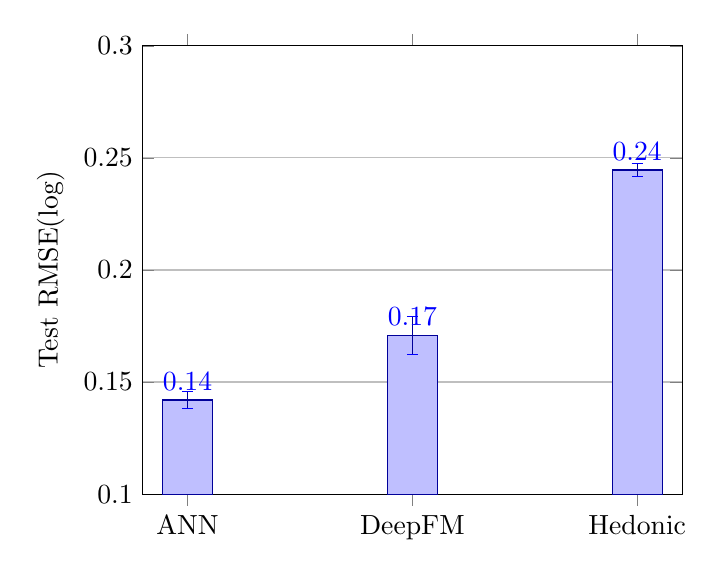
\begin{tikzpicture}
\begin{axis}[
  ybar,
  bar width=18pt,
  ylabel={Test RMSE(log)},
  symbolic x coords={ANN,DeepFM,Hedonic},
  xtick=data,
  ymin=0.10, ymax=0.30,
  ymajorgrids=true,
  error bars/y dir=both,
  error bars/y explicit,
  nodes near coords,
  nodes near coords align={vertical},
]
\addplot+[fill=blue!25, draw=blue!60!black] coordinates {
  (ANN,\AnnRandRmseMean) +- (0,\AnnRandRmseStd)
  (DeepFM,\DeepRandRmseMean) +- (0,\DeepRandRmseStd)
  (Hedonic,\HedRandRmseMean) +- (0,\HedRandRmseStd)
};
\end{axis}
\end{tikzpicture}
\caption{RMSE(log) on random split.}
\end{subfigure}
\hfill
\begin{subfigure}{0.49\linewidth}
\centering
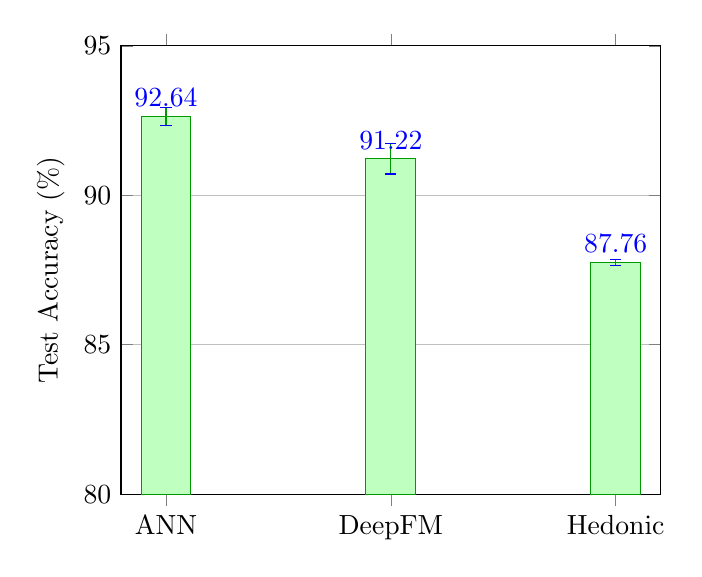
\begin{tikzpicture}
\begin{axis}[
  ybar,
  bar width=18pt,
  ylabel={Test Accuracy (\%)},
  symbolic x coords={ANN,DeepFM,Hedonic},
  xtick=data,
  ymin=80, ymax=95,
  ymajorgrids=true,
  error bars/y dir=both,
  error bars/y explicit,
  nodes near coords,
  nodes near coords align={vertical},
]
\addplot+[fill=green!25, draw=green!60!black] coordinates {
  (ANN,\AnnRandAccMean) +- (0,\AnnRandAccStd)
  (DeepFM,\DeepRandAccMean) +- (0,\DeepRandAccStd)
  (Hedonic,\HedRandAccMean) +- (0,\HedRandAccStd)
};
\end{axis}
\end{tikzpicture}
\caption{Accuracy\% on random split.}
\end{subfigure}
\caption{Random-split performance (mean $\pm$ std). ANN/Hedonic statistics are from \texttt{eval\_suite} runs; DeepFM statistics are from 3 full-train seeds (0/1/42).}
\label{fig:random-bars}
\end{figure}

\subsection{Time split: mean $\pm$ std across seeds}
\begin{figure}[h]
\centering
\begin{subfigure}{0.49\linewidth}
\centering
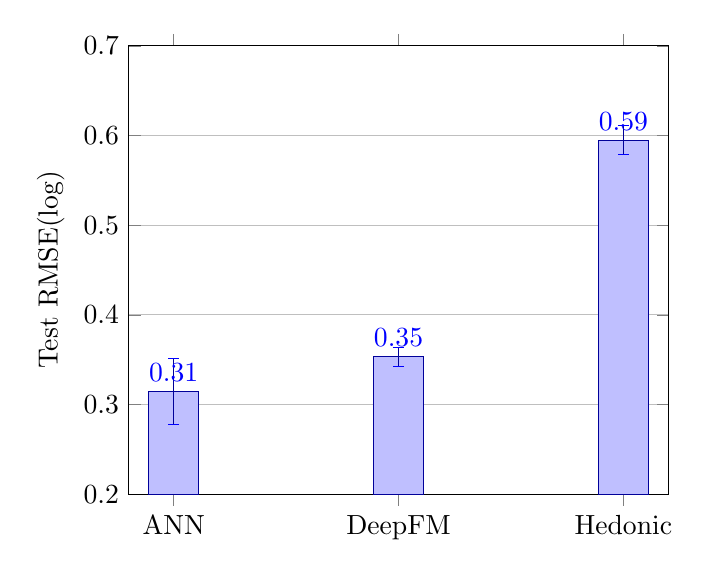
\begin{tikzpicture}
\begin{axis}[
  ybar,
  bar width=18pt,
  ylabel={Test RMSE(log)},
  symbolic x coords={ANN,DeepFM,Hedonic},
  xtick=data,
  ymin=0.20, ymax=0.70,
  ymajorgrids=true,
  error bars/y dir=both,
  error bars/y explicit,
  nodes near coords,
  nodes near coords align={vertical},
]
\addplot+[fill=blue!25, draw=blue!60!black] coordinates {
  (ANN,\AnnTimeRmseMean) +- (0,\AnnTimeRmseStd)
  (DeepFM,\DeepTimeRmseMean) +- (0,\DeepTimeRmseStd)
  (Hedonic,\HedTimeRmseMean) +- (0,\HedTimeRmseStd)
};
\end{axis}
\end{tikzpicture}
\caption{RMSE(log) on time split.}
\end{subfigure}
\hfill
\begin{subfigure}{0.49\linewidth}
\centering
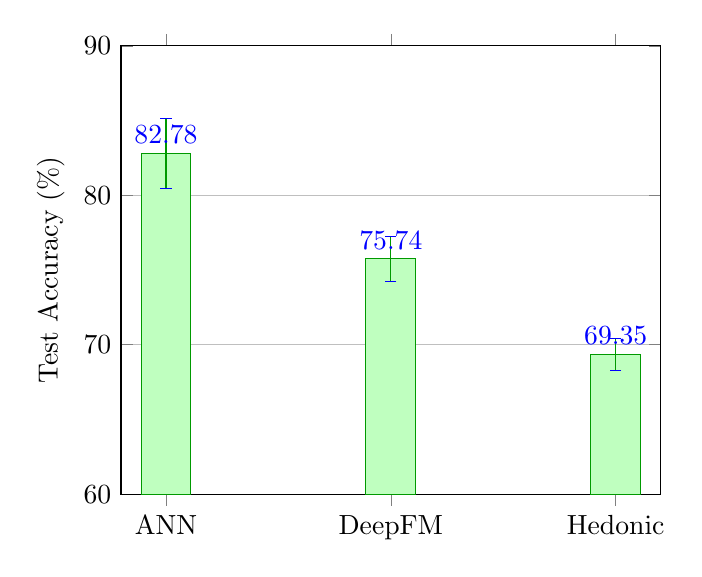
\begin{tikzpicture}
\begin{axis}[
  ybar,
  bar width=18pt,
  ylabel={Test Accuracy (\%)},
  symbolic x coords={ANN,DeepFM,Hedonic},
  xtick=data,
  ymin=60, ymax=90,
  ymajorgrids=true,
  error bars/y dir=both,
  error bars/y explicit,
  nodes near coords,
  nodes near coords align={vertical},
]
\addplot+[fill=green!25, draw=green!60!black] coordinates {
  (ANN,\AnnTimeAccMean) +- (0,\AnnTimeAccStd)
  (DeepFM,\DeepTimeAccMean) +- (0,\DeepTimeAccStd)
  (Hedonic,\HedTimeAccMean) +- (0,\HedTimeAccStd)
};
\end{axis}
\end{tikzpicture}
\caption{Accuracy\% on time split.}
\end{subfigure}
\caption{Time-split performance (mean $\pm$ std). Time splits are harder; ANN retains a large advantage over the hedonic baseline and also outperforms DeepFM in these runs.}
\label{fig:time-bars}
\end{figure}

\section{Seed sensitivity under a time-based split}
Time-based evaluation is substantially more sensitive to initialization than the random split. Figures~\ref{fig:time-seed-ann}--\ref{fig:time-seed-hed} plot time-split test metrics for each model seed under two time-ordering tiebreak settings (\texttt{split\_seed} = 42 vs 7).

\begin{figure}[h]
\centering
\begin{subfigure}{0.49\linewidth}
\centering
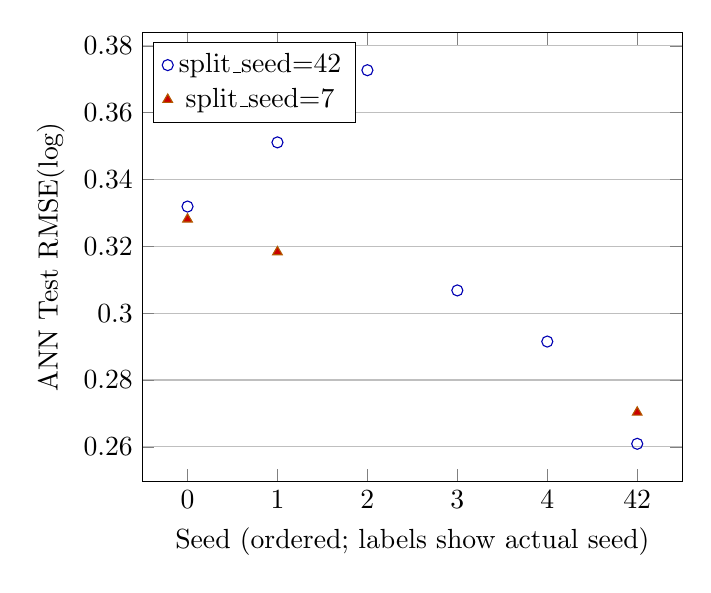
\begin{tikzpicture}
\begin{axis}[
  xlabel={Seed (ordered; labels show actual seed)},
  ylabel={ANN Test RMSE(log)},
  xmin=-0.5, xmax=5.5,
  xtick={0,1,2,3,4,5},
  xticklabels={0,1,2,3,4,42},
  ymajorgrids=true,
  legend style={at={(0.02,0.98)},anchor=north west},
]
\addplot+[only marks, mark=o, color=blue!70!black] coordinates {
  (0,0.3319) (1,0.3511) (2,0.3727) (3,0.3068) (4,0.2915) (5,0.2609)
};
\addlegendentry{split\_seed=42}
\addplot+[only marks, mark=triangle*, color=orange!70!black] coordinates {
  (0,0.3281) (1,0.3183) (5,0.2703)
};
\addlegendentry{split\_seed=7}
\end{axis}
\end{tikzpicture}
\caption{ANN time-split RMSE(log).}
\end{subfigure}
\hfill
\begin{subfigure}{0.49\linewidth}
\centering
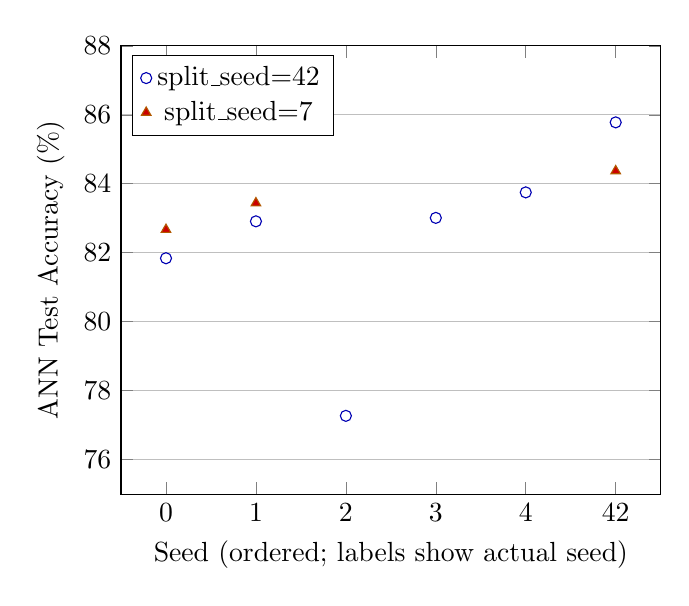
\begin{tikzpicture}
\begin{axis}[
  xlabel={Seed (ordered; labels show actual seed)},
  ylabel={ANN Test Accuracy (\%)},
  xmin=-0.5, xmax=5.5,
  xtick={0,1,2,3,4,5},
  xticklabels={0,1,2,3,4,42},
  ymin=75, ymax=88,
  ymajorgrids=true,
  legend style={at={(0.02,0.98)},anchor=north west},
]
\addplot+[only marks, mark=o, color=blue!70!black] coordinates {
  (0,81.84) (1,82.91) (2,77.27) (3,83.01) (4,83.75) (5,85.78)
};
\addlegendentry{split\_seed=42}
\addplot+[only marks, mark=triangle*, color=orange!70!black] coordinates {
  (0,82.67) (1,83.44) (5,84.37)
};
\addlegendentry{split\_seed=7}
\end{axis}
\end{tikzpicture}
\caption{ANN time-split accuracy.}
\end{subfigure}
\caption{ANN sensitivity under time-based evaluation. The best observed run here is seed=42 with \texttt{split\_seed}=42 (RMSE=0.2609, Acc=85.78\%).}
\label{fig:time-seed-ann}
\end{figure}

\begin{figure}[h]
\centering
\begin{subfigure}{0.49\linewidth}
\centering
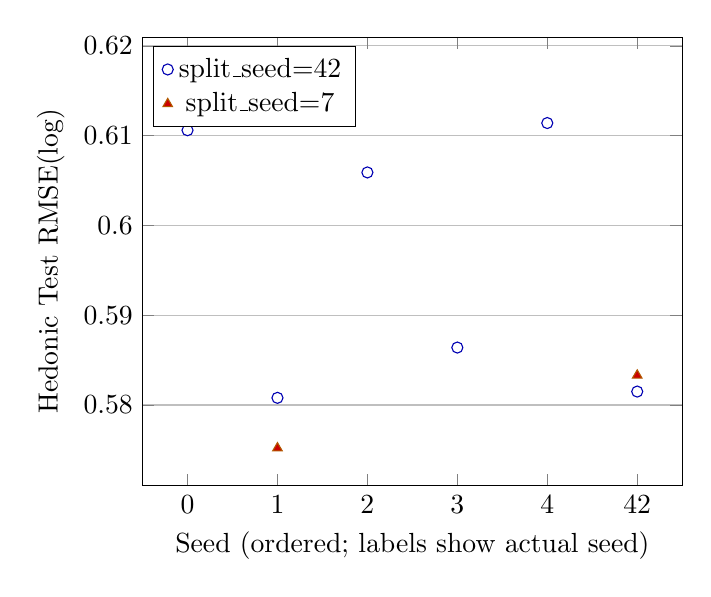
\begin{tikzpicture}
\begin{axis}[
  xlabel={Seed (ordered; labels show actual seed)},
  ylabel={Hedonic Test RMSE(log)},
  xmin=-0.5, xmax=5.5,
  xtick={0,1,2,3,4,5},
  xticklabels={0,1,2,3,4,42},
  ymajorgrids=true,
  legend style={at={(0.02,0.98)},anchor=north west},
]
\addplot+[only marks, mark=o, color=blue!70!black] coordinates {
  (0,0.6106) (1,0.5808) (2,0.6059) (3,0.5864) (4,0.6114) (5,0.5815)
};
\addlegendentry{split\_seed=42}
\addplot+[only marks, mark=triangle*, color=orange!70!black] coordinates {
  (0,0.6168) (1,0.5752) (5,0.5833)
};
\addlegendentry{split\_seed=7}
\end{axis}
\end{tikzpicture}
\caption{Hedonic time-split RMSE(log).}
\end{subfigure}
\hfill
\begin{subfigure}{0.49\linewidth}
\centering
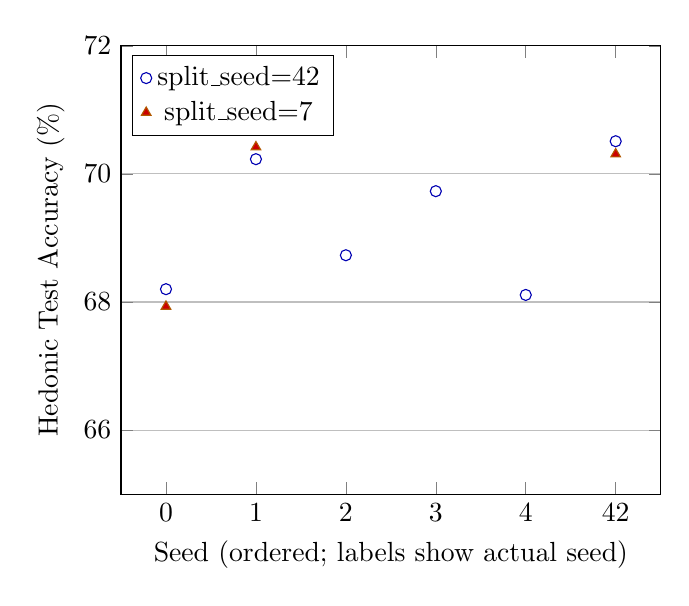
\begin{tikzpicture}
\begin{axis}[
  xlabel={Seed (ordered; labels show actual seed)},
  ylabel={Hedonic Test Accuracy (\%)},
  xmin=-0.5, xmax=5.5,
  xtick={0,1,2,3,4,5},
  xticklabels={0,1,2,3,4,42},
  ymin=65, ymax=72,
  ymajorgrids=true,
  legend style={at={(0.02,0.98)},anchor=north west},
]
\addplot+[only marks, mark=o, color=blue!70!black] coordinates {
  (0,68.20) (1,70.23) (2,68.73) (3,69.73) (4,68.11) (5,70.51)
};
\addlegendentry{split\_seed=42}
\addplot+[only marks, mark=triangle*, color=orange!70!black] coordinates {
  (0,67.93) (1,70.42) (5,70.31)
};
\addlegendentry{split\_seed=7}
\end{axis}
\end{tikzpicture}
\caption{Hedonic time-split accuracy.}
\end{subfigure}
\caption{Hedonic sensitivity under time-based evaluation. Performance is much lower than ANN and DeepFM under time splits.}
\label{fig:time-seed-hed}
\end{figure}

\section{Sweep trade-offs (sampled points)}
Large sweeps (ANN deep-test, FM, DeepFM, TabNet) often cap training rows to 50,000 for speed. Figure~\ref{fig:sweep-scatter} shows a random sample of sweep runs (filtered to a reasonable accuracy range) to illustrate the typical RMSE/accuracy trade-off across model families.

\begin{figure}[h]
\centering
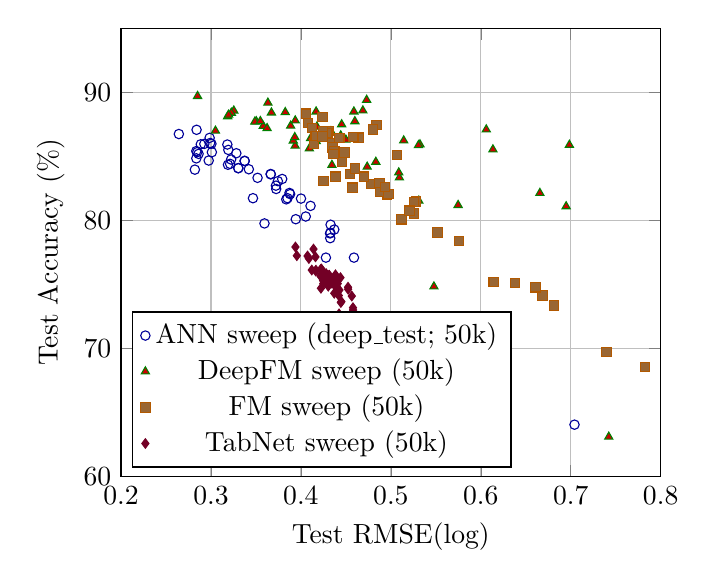
\begin{tikzpicture}
\begin{axis}[
  xlabel={Test RMSE(log)},
  ylabel={Test Accuracy (\%)},
  xmin=0.20, xmax=0.80,
  ymin=60, ymax=95,
  grid=both,
  legend style={at={(0.02,0.02)},anchor=south west},
]
\addplot+[only marks, mark=o, mark size=1.7pt, color=blue!60!black] coordinates {
  (0.3792,83.23) (0.3873,82.14) (0.3189,84.34) (0.4278,77.09) (0.3193,85.50) (0.3518,83.32) (0.4107,81.13) (0.3010,85.32) (0.2840,87.07) (0.3182,85.92) (0.3467,81.73) (0.2887,85.94) (0.3851,81.73) (0.3304,84.08) (0.3665,83.59) (0.2837,85.41) (0.3837,81.64) (0.3725,82.45) (0.7042,64.05) (0.2837,84.84) (0.3304,84.07) (0.4328,79.03) (0.2991,86.04) (0.3943,80.09) (0.3005,85.98) (0.4001,81.70) (0.2643,86.74) (0.2821,83.96) (0.3595,79.76) (0.3374,84.65) (0.3421,83.99) (0.2926,85.97) (0.4590,77.09) (0.2862,85.19) (0.2975,84.67) (0.3375,84.63) (0.3282,85.24) (0.3213,84.41) (0.4054,80.30) (0.3880,82.05) (0.3664,83.62) (0.4326,78.61) (0.2985,86.44) (0.4330,79.66) (0.3224,84.75) (0.2848,85.33) (0.3722,82.71) (0.3744,83.06) (0.4371,79.28) (0.4324,78.98)
};
\addlegendentry{ANN sweep (deep\_test; 50k)}

\addplot+[only marks, mark=triangle*, mark size=1.7pt, color=green!50!black] coordinates {
  (0.5095,83.34) (0.3186,88.12) (0.5324,85.92) (0.5143,86.23) (0.4731,89.40) (0.4600,87.73) (0.3504,87.73) (0.4737,84.18) (0.3254,88.56) (0.6985,85.89) (0.4589,88.49) (0.4169,88.49) (0.2851,89.70) (0.3936,85.82) (0.3050,86.99) (0.3886,87.38) (0.5307,85.86) (0.3937,87.79) (0.3226,88.39) (0.4094,85.61) (0.4500,86.29) (0.4833,84.56) (0.4453,87.49) (0.4178,87.31) (0.5516,69.10) (0.6061,87.09) (0.3488,87.70) (0.4443,86.62) (0.3196,88.24) (0.3672,88.41) (0.5748,81.19) (0.4170,86.18) (0.3633,89.18) (0.4689,88.57) (0.3581,87.36) (0.3826,88.44) (0.6657,82.13) (0.6949,81.09) (0.3624,87.19) (0.3549,87.74) (0.5479,74.83) (0.4334,86.95) (0.4345,84.32) (0.5311,81.53) (0.6135,85.53) (0.4108,86.41) (0.3915,86.22) (0.3932,86.49) (0.5088,83.73) (0.7423,63.10)
};
\addlegendentry{DeepFM sweep (50k)}

\addplot+[only marks, mark=square*, mark size=1.7pt, color=orange!70!black] coordinates {
  (0.4840,87.44) (0.4351,86.00) (0.5256,80.54) (0.4959,81.99) (0.4779,82.83) (0.4880,82.26) (0.5518,79.05) (0.4801,87.10) (0.7397,69.72) (0.5069,85.11) (0.5118,80.08) (0.4056,88.33) (0.4547,83.62) (0.4077,87.59) (0.4485,85.29) (0.4146,86.00) (0.5282,81.49) (0.4352,85.70) (0.4309,86.97) (0.4874,82.92) (0.6815,73.36) (0.6144,75.17) (0.5260,81.44) (0.4427,86.44) (0.4363,85.18) (0.4126,87.22) (0.4386,83.41) (0.5207,80.75) (0.4241,88.06) (0.4371,85.37) (0.4456,84.56) (0.4974,82.07) (0.4293,86.80) (0.6383,75.12) (0.4604,84.04) (0.4245,86.98) (0.4643,86.45) (0.4572,82.55) (0.6687,74.13) (0.4364,85.18) (0.7828,68.57) (0.4164,86.58) (0.4702,83.41) (0.4974,82.07) (0.4252,83.09) (0.5756,78.38) (0.6609,74.77) (0.4937,82.61) (0.4582,86.51) (0.4240,86.55)
};
\addlegendentry{FM sweep (50k)}

\addplot+[only marks, mark=diamond*, mark size=1.7pt, color=purple!60!black] coordinates {
  (0.4140,77.76) (0.4450,73.66) (0.4220,76.17) (0.4344,75.10) (0.4389,74.78) (0.4706,71.86) (0.4089,77.02) (0.4220,75.63) (0.4223,74.70) (0.4228,76.20) (0.4390,75.01) (0.4428,74.56) (0.4281,75.84) (0.4395,75.23) (0.4386,75.52) (0.4074,77.22) (0.4580,73.00) (0.4281,75.47) (0.4398,75.47) (0.4566,74.09) (0.3939,77.92) (0.4424,72.70) (0.4444,73.59) (0.4384,75.75) (0.4342,75.42) (0.4524,74.78) (0.4284,75.10) (0.4121,76.12) (0.4371,74.31) (0.4304,74.86) (0.4535,72.07) (0.4229,76.17) (0.4421,74.13) (0.4579,73.18) (0.4249,75.06) (0.3955,77.24) (0.4519,71.99) (0.4253,75.73) (0.4218,75.68) (0.4409,75.06) (0.4440,75.53) (0.4309,75.69) (0.4247,75.29) (0.4167,76.11) (0.4525,74.62) (0.4782,71.62) (0.4164,76.05) (0.4316,75.71) (0.4379,74.97) (0.4162,77.15)
};
\addlegendentry{TabNet sweep (50k)}
\end{axis}
\end{tikzpicture}
\caption{Sampled sweep runs (full features, random split). Sweeps cap training rows for speed; full-train ANN/DeepFM runs still outperform these sweeps.}
\label{fig:sweep-scatter}
\end{figure}

\section{Feature importance (permutation analysis)}
To interpret model improvements, we compute permutation feature importance on a validation subset (20k rows) by measuring the increase in validation MSE when permuting one feature at a time.

\begin{figure}[h]
\centering
\begin{subfigure}{0.49\linewidth}
\centering
\begin{tikzpicture}
\begin{axis}[
  xbar,
  xlabel={Increase in validation MSE (Δval\_mse)},
  ytick=data,
  yticklabels={
    numeric:LivingArea,
    numeric:TransactionYear,
    categorical:FSA,
    categorical:gcode\_City,
    numeric:YearBuilt,
    categorical:BuildingType,
    categorical:Ownership,
    categorical:PropertyStyle,
    numeric:gcode\_Lon,
    numeric:gcode\_Lat
  },
  ymin=-0.5, ymax=9.5,
  height=8cm,
  grid=both,
]
\addplot+[fill=blue!25, draw=blue!60!black] coordinates {
  (0.098610,0) (0.089895,1) (0.066793,2) (0.042350,3) (0.011641,4)
  (0.009254,5) (0.007690,6) (0.006414,7) (0.006256,8) (0.005573,9)
};
\end{axis}
\end{tikzpicture}
\caption{ANN top-10 features.}
\end{subfigure}
\hfill
\begin{subfigure}{0.49\linewidth}
\centering
\begin{tikzpicture}
\begin{axis}[
  xbar,
  xlabel={Increase in validation MSE (Δval\_mse)},
  ytick=data,
  yticklabels={
    numeric:LivingArea,
    categorical:FSA,
    numeric:TransactionYear,
    categorical:gcode\_City,
    numeric:gcode\_Lon,
    categorical:PropertyStyle,
    categorical:Ownership,
    categorical:BuildingType,
    numeric:Bath\_Full,
    categorical:Basement
  },
  ymin=-0.5, ymax=9.5,
  height=8cm,
  grid=both,
]
\addplot+[fill=orange!25, draw=orange!70!black] coordinates {
  (0.096493,0) (0.072510,1) (0.064920,2) (0.021628,3) (0.016773,4)
  (0.006725,5) (0.005359,6) (0.005347,7) (0.004804,8) (0.003832,9)
};
\end{axis}
\end{tikzpicture}
\caption{Hedonic top-10 features.}
\end{subfigure}
\caption{Permutation feature importance (validation subset). Location and time variables are major drivers; ANN shows stronger gains from nonlinear and interaction-heavy signals.}
\label{fig:feature-importance}
\end{figure}

\section{Discussion}
\paragraph{Why the ANN outperforms hedonic regression.}
Both models benefit strongly from adding time and location signals (e.g.\ \texttt{TransactionYear}, \texttt{FSA}, \texttt{gcode\_City}, lat/lon). The ANN improves further by learning nonlinear effects and interactions (e.g.\ diminishing returns to size, location-dependent trends, and cross-feature interactions) that a linear hedonic model cannot represent.

\paragraph{Random vs time splits.}
Random splits measure interpolation across mixed time periods; time splits are closer to a forecasting evaluation. Performance drops notably under time splits for all models, but the ANN retains a large advantage (\(\approx\) 13.4 percentage points higher test accuracy than the hedonic baseline on average in our time-split checks).

\section{Limitations and next steps}
\begin{itemize}[leftmargin=*]
  \item \textbf{Preprocessing leakage:} current tensorization computes numeric mean/std and categorical vocab using the full dataset. A stricter setup would compute these on training data only per split.
  \item \textbf{Sweep hygiene:} \texttt{sweep\_ann\_deep\_test.py} evaluates test every run and should be treated as exploratory; \texttt{sweep\_ann.py} is the test-clean sweep.
  \item \textbf{Boosting baselines:} run XGBoost/LightGBM externally using \texttt{models/06\_xgboost/train\_boosting.py}, then merge \texttt{xgb\_runs.csv}/\texttt{lgbm\_runs.csv} into \texttt{results\_all.csv} via \texttt{export\_results.py}.
  \item \textbf{Interpretability:} extend feature analysis (e.g.\ partial dependence-style perturbations) on top drivers such as \texttt{LivingArea} and \texttt{TransactionYear}.
\end{itemize}

\section*{Reproducibility pointers}
\begin{itemize}[leftmargin=*]
  \item Canonical results sheet: \texttt{results\_all.csv}
  \item Interactive dashboard (download buttons included): \texttt{plots/report\_graphs.html}
  \item Merge all intermediate logs into the canonical sheet: \texttt{python export\_results.py}
\end{itemize}

\begin{thebibliography}{9}
\bibitem{rendle2010fm}
Steffen Rendle.
\newblock Factorization Machines.
\newblock In \emph{ICDM}, 2010.

\bibitem{guo2017deepfm}
Huifeng Guo, Ruiming Tang, Yunming Ye, Zhenguo Li, Xiuqiang He.
\newblock DeepFM: A Factorization-Machine based Neural Network for CTR Prediction.
\newblock In \emph{IJCAI}, 2017.

\bibitem{arik2019tabnet}
Sercan O. Arik, Tomas Pfister.
\newblock TabNet: Attentive Interpretable Tabular Learning.
\newblock \emph{arXiv:1908.07442}, 2019.

\bibitem{chen2016xgboost}
Tianqi Chen, Carlos Guestrin.
\newblock XGBoost: A Scalable Tree Boosting System.
\newblock In \emph{KDD}, 2016.

\bibitem{ke2017lightgbm}
Guolin Ke et al.
\newblock LightGBM: A Highly Efficient Gradient Boosting Decision Tree.
\newblock In \emph{NeurIPS}, 2017.
\end{thebibliography}

\end{document}
